% SSEE — Unified Journal Paper
% Target: JCAP / PRD / Universe (MDPI)
% Compile: pdflatex (×2) + bibtex + pdflatex (×2)
\documentclass[12pt,a4paper]{article}

\usepackage[utf8]{inputenc}
\usepackage{amsmath,amssymb,amsfonts}
\usepackage{graphicx}
\usepackage{booktabs}
\usepackage[colorlinks=true,linkcolor=red!70!black,citecolor=green!50!black,urlcolor=blue!80!black]{hyperref}
\usepackage{xcolor}
\usepackage{geometry}
\usepackage{natbib}
\usepackage{caption}
\usepackage{float}
\usepackage{array}
\usepackage{tabularx}
\usepackage{enumitem}
\usepackage{tcolorbox}
\usepackage{multirow}
\geometry{margin=2.5cm}
\emergencystretch=2em

% ─── Macros ──────────────────────────────────────────────────────────────────
\newcommand{\SSEE}{\textsc{ssee}}
\newcommand{\LCDM}{$\Lambda$CDM}
\newcommand{\phiG}{\varphi}
\newcommand{\KAL}{\mathrm{KAL}_0}
\newcommand{\MIRA}{\mathcal{M}}
\newcommand{\AURA}{\mathrm{AURA}}
\newcommand{\thetaE}{\theta_E}
\newcommand{\fscr}{f_{\mathrm{scr}}}
\newcommand{\Omde}{\Omega_{\mathrm{DE}}}
\newcommand{\Omm}{\Omega_{m}}
\newcommand{\Ommdyn}{\Omega_{m,\mathrm{dyn}}}
\newcommand{\OmmCMB}{\Omega_{m,\mathrm{CMB}}}
\newcommand{\wz}{w_0}
\newcommand{\wa}{w_a}
\newcommand{\sig}{\sigma_8}
\newcommand{\sigeff}{\sigma_8^{\mathrm{eff}}}
\newcommand{\kfs}{k_{\mathrm{fs}}}
\newcommand{\mphi}{m_\phi}
\newcommand{\fsig}{f\sigma_8}
\newcommand{\alphaK}{\alpha_K}
\newcommand{\alphaB}{\alpha_B}
\newcommand{\alphaM}{\alpha_M}
\newcommand{\alphaT}{\alpha_T}
\newcommand{\half}{\tfrac{1}{2}}
\newcommand{\GR}{\mathrm{GR}}

% ─────────────────────────────────────────────────────────────────────────────
\title{\textbf{Structural Self-Energy Expansion (SSEE):\\
A Minimal-Parameter Dark Energy Framework ---\\
Algebraic Derivation, Boltzmann Validation, and\\
Effective Field Theory Stability Analysis}}

\author{Mike Edison Almeida Vallejo \\
\small \textit{Independent Researcher} \\
\small \href{mailto:mike.almeida1721@gmail.com}{mike.almeida1721@gmail.com} \\
\small ORCID: \href{https://orcid.org/0009-0008-2195-7836}{0009-0008-2195-7836}
}

\date{May 2026}

% ─────────────────────────────────────────────────────────────────────────────
\sloppy
\begin{document}

\maketitle

% ─── Abstract ────────────────────────────────────────────────────────────────
\begin{abstract}
We present the Structural Self-Energy Expansion (\SSEE), a dark energy
framework that derives its cosmological background sector algebraically
from the golden ratio $\phiG$ and $\pi$, with zero fitted dimensionless
parameters at the background level and no WIMP, QCD-axion, or SUSY dark-matter
particle. Phenomenological extensions in the dark-matter sector, proposed in an
earlier version of Paper~6, are \emph{retracted} (\S\ref{sec:growth_raw}): the
matter sector is a single unpartitioned component, and their register entries
(OP-9, OP-11) close by dissolution (\texttt{OPEN\_PROBLEMS.md}). In CMB-likelihood terms SSEE is a $k=2$ fit: of
$\Lambda$CDM's six parameters it fixes four algebraically ($\Omega_b$, $\Omega_c$
via $\omega_c=\mathrm{KAL}_0\,\omega_b\,n_s$, $n_s=1-\phiG^{-7}$, and the derived
anchor $H_0/(\mathrm{km\,s^{-1}\,Mpc^{-1}})=3(\phiG+\pi)^2$), leaving only the primordial amplitude $A_s$ and the
optical depth $\tau$ ($k=2$ versus $k=6$, the count used in the Paper~3 model
comparison).
The dark energy equation of state $\wz = -(3\phiG+\pi)/[2(\phiG+\pi)] \simeq -0.840$
and $\wa \simeq -0.670$ are fixed by the algebraic construction and agree with the
official DESI~DR2 $w_0w_a$CDM posterior within $0.24\sigma$ (Pantheon+;
$0.2$--$1.8\sigma$ across SN compilations)---a parameter-free postdiction, with no
claim of temporal priority over DESI~DR2.
A Bayesian MCMC analysis under the $\omega_m$-direct CMB anchor as prior
($H_0^{\rm prior,SSEE}=67.96214\pm0.54$~km\,s$^{-1}$\,Mpc$^{-1}$, the value at
which Planck~\texttt{plik\_lite} is minimised with SSEE-fixed $\omega_b,\omega_c$; Paper~3) yields
$H_0 = 67.79^{+0.35}_{-0.35}$~km\,s$^{-1}$\,Mpc$^{-1}$ ($0.66\sigma$ from Planck,
$0.50\sigma$ from the algebraic anchor) and $\Delta\mathrm{BIC}=6.43$ favouring
\SSEE\ over \LCDM\ ($6.35$ over CPL).
A complementary full-likelihood multi-probe MCMC (CAMB $+$ Planck
\texttt{plik\_lite} $+$ lensing $+$ DESI~DR2 $+$ $f\sigma_8$, $w_0,w_a$ free and
$H_0$ under a flat prior) places the model at $1.31\sigma$ in the $w_0$--$w_a$
plane, where \LCDM\ is excluded at $3.22\sigma$; under this uncompressed CMB
likelihood $H_0$ relaxes to $65.87\pm1.17$ ($1.79\sigma$ below the anchor).

The CMB-sector matter density is the standard physical observable
$\OmmCMB = \omega_m/h^2 = 0.308881$ (Planck: $0.3153\pm 0.0073$), built
piece-by-piece from SSEE algebra ($\omega_m$-direct; OP-8 dissolved, no matter
factor) and distinct from the dynamical $\Ommdyn = 0.160050$ that governs DESI BAO.
Full-sky CLASS Boltzmann runs confirm that the \emph{full} matter density is
physically necessary: using only $\Ommdyn=0.160050$ as the CMB matter density
shifts the peak positions by $\sim 10\%$ and raises the RMS residual
from $1.4\%$ to $31.5\%$.

A linear Israel-Stewart perturbation analysis with $\Omega_{m,\mathrm{cosm}}=0.308881$ in
the Poisson equation yields a growth factor
$\mathcal{G} = 1.0032$ and $\sigma_8 = 0.8136$ (Paper~5), giving a mean
$\fsig$ tension of $0.70\sigma$ across six RSD surveys --- statistically identical
to $\Lambda$CDM ($0.73\sigma$), resolving the growth-rate sector.
In the lensing amplitude, fitting the primordial amplitude to the $225$
\emph{raw} KiDS-1000 $\xi_\pm$ data points with a \emph{single} unpartitioned
matter sector and the background fixed by the algebra gives
$\sigma_8=0.7446\pm0.0189$ and $S_8=0.7555\pm0.0192$ (the $\Lambda$CDM control on the same raw data gives $0.7571\pm0.0194$), i.e.\ $0.11\sigma$ from
KiDS-1000: \textbf{no $S_8$ tension} (\S\ref{sec:growth_raw}). A two-sector
$\phi$-DM extension previously reported here is \emph{retracted} ---
the deliberate cost of lowering $\sigma_8$ to resolve the lensing amplitude.

An EFTCAMB validation at the Bellini-Sawicki level uses the fluid-approximation
input $\alphaK^{\rm eff} = 0.403302$ ($\Delta = 0.005\%$), while the theoretical
bare-field value is $\alphaK = 0.072567$ (Paper~7), with $\alphaT = \alphaM = \alphaB = 0$
(GW170817 compatible) and strictly positive kinetic stability ($Q_s > 0$).

We additionally summarise three theoretical extensions of the framework.
In the strong-field regime Paper~8 analyses two limits: an alternative
MOND-like limit in which the photon deflection is amplified by
$\sqrt{\AURA}\approx 1.9995$ (numerically close to $\MIRA$ at $0.03\%$ but
algebraically distinct), and the canonical limit with EFT
$\alpha_B=\alpha_M=\alpha_T=0$ in which the residual fifth-force is
suppressed to $F_\phi/F_N\sim 10^{-15}$ and the observable lensing recovers
GR; current SLACS/BELLS data favour the canonical limit (Paper~8;
OPEN\_PROBLEMS.md OP-13). A late-time local screening fraction
$f_{\rm scr}^{\rm IR}=\alphaK/(3\MIRA)=(\pi-\phiG)/(\phiG+\pi)^2\simeq0.067$ relates
the locally measured rate to the global background. The measured datum is the
input and the global rate is the output:
$H_0^{\rm glob}=H_0^{\rm SH0ES}(1-f_{\rm scr}^{\rm IR})=68.13$~km\,s$^{-1}$\,Mpc$^{-1}$,
which sits $0.17\sigma$ from the pure number $3(\phiG+\pi)^2=67.96214$; with the
full infrared-plus-ultraviolet fraction $f_{\rm scr}^{\rm full}=0.069522$ the same
operation returns $67.962142$, a residual of $+4.2\times10^{-6}$ against that
number, in both cases with zero free parameters (Papers~9 and~10).
A UV completion $K(X)=X/\KAL+X^2/M^4$ with algebraic cutoff $M=9.68$~meV
connects the dark-energy EFT to the inflationary $\alpha$-attractor (Paper~10).
All model parameters are falsifiable by named forthcoming experiments.
\end{abstract}

\clearpage
\tableofcontents
\clearpage
\newpage

% ─────────────────────────────────────────────────────────────────────────────
\section{Introduction}
\label{sec:intro}
% ─────────────────────────────────────────────────────────────────────────────

The DESI~DR2 baryon acoustic oscillation data \citep{AbdulKarim2025} provide
compelling evidence for dynamical dark energy at $>3\sigma$, with a CPL
equation-of-state posterior centred near $(\wz,\wa) \approx (-0.84, -0.67)$.
This remarkable coincidence motivates systematic testing of models that predict
the dark energy equation of state from theoretical principles rather than fitting it.

The \SSEE framework proposes that the macroscopic universe obeys an
algebraic closure condition: all cosmological background parameters are uniquely
determined by two dimensionless geometric constants, the golden ratio
$\phiG = (1+\sqrt{5})/2 \simeq 1.6180$ and $\pi \simeq 3.1416$.
No optimisation over formula space was performed: the parameter values are fixed
by the algebraic construction \citep{AlmeidaSSEE2026genesis}, not adjusted to the
data. We make no claim of temporal priority over DESI~DR2 (public from 2025 March);
the agreement reported below is a parameter-free \emph{postdiction}, and the only
timestamped predictions are those reserved for unreleased data (DESI~DR3, Euclid).

This paper consolidates the complete \SSEE\ validation programme across
ten companion preprints \citep{AlmeidaSSEE2026P1,AlmeidaSSEE2026P2,
AlmeidaSSEE2026P3,AlmeidaSSEE2026P4,AlmeidaSSEE2026P5,AlmeidaSSEE2026P6,
AlmeidaSSEE2026P7,AlmeidaSSEE2026P8,AlmeidaSSEE2026P9,AlmeidaSSEE2026P10}
into a single self-contained presentation.
We report four independent validation tiers:
\begin{enumerate}[leftmargin=*,itemsep=1pt]
\item \textbf{Background sector} (\S\ref{sec:background}): Bayesian MCMC
  against DESI~DR2 BAO, a compressed Planck~2018 prior, and galaxy-cluster
  dynamical masses.
\item \textbf{CMB angular spectrum} (\S\ref{sec:cmb}): Full-sky CLASS Boltzmann
  integration demonstrating that the full $\omega_m$-direct matter density
  ($\OmmCMB=0.308881$) is physically necessary for reproducing Planck~PR4 peak positions.
\item \textbf{Structure growth and $\sigma_8$} (\S\ref{sec:growth}): Israel-Stewart
  causal perturbation theory with a single matter sector. The $S_8$ ``tension''
  is shown to be an artefact of fixing $A_s$ to Planck: with $A_s$ free, the MCMC
  against raw KiDS-1000 $\xi_\pm$ gives $S_8=0.7555\pm0.0192$, $0.11\sigma$. The
  earlier $\phi$-DM two-sector extension is retired (2026-08-01). (Formerly $\sim0.2\sigma$
  cost in $\fsig$, which rises to $0.93\sigma$).
\item \textbf{EFT stability} (\S\ref{sec:eft}): EFTCAMB Bellini-Sawicki
  validation of kinetic stability ($\alphaK$) and gravitational wave compatibility
  ($\alphaT = \alphaM = \alphaB = 0$).
\end{enumerate}
Section~\ref{sec:extensions} then summarises three theoretical extensions of the
framework --- the strong-field lensing regime, an algebraic resolution of the
Hubble tension, and a UV completion --- which are developed in full in the
companion Papers~8--10 and are presented here in condensed form.

Throughout, we distinguish three epistemic statuses: \textit{postdiction}
(algebraic result fixed by construction, then compared to data already public),
\textit{retrodiction} (independently derived, then compared to existing data),
and \textit{prediction} (fixed now, tested against not-yet-released data).
Table~\ref{tab:register} in \S\ref{sec:falsify} lists all entries explicitly.


% ─────────────────────────────────────────────────────────────────────────────
\section{Algebraic Framework}
\label{sec:theory}
% ─────────────────────────────────────────────────────────────────────────────

\subsection{Structural registers}
\label{sec:registers}

The \SSEE\ framework postulates a closed algebraic system of seven structural
registers derived from $\phiG$ and $\pi$:
\begin{align}
  \Omega   &= \pi + \phiG                   \simeq 4.7596 \quad (\text{Stability Metric})  \nonumber\\
  \beta    &= (\pi + \phiG)/2               \simeq 2.3798 \quad (\text{Base Coupling Scalar}) \nonumber\\
  \KAL     &= \beta + \pi                   \simeq 5.5214 \quad (\text{Structural Retention}) \nonumber\\
  P_{\rm sc} &= \Omega + \phiG             \simeq 6.3777 \quad (\text{Dynamical Evolution Scalar}) \nonumber\\
  K_v      &= \phiG + \pi + \Omega         \simeq 9.5193 \quad (\text{Structural Constraint}) \nonumber\\
  T_r      &= 3(\phiG + \beta)             \simeq 11.9935\quad (\text{3D Saturation Horizon}) \nonumber\\
  M_v      &= \phiG + \pi + K_v           \simeq 14.2789\quad (\text{Maximal Dimensional Invariant})
  \label{eq:registers}
\end{align}
From these seven scalars, the dark energy equation of state is derived uniquely:
\begin{equation}
  \wz = -\frac{T_r}{M_v}
     = -\frac{3\phiG+\pi}{2(\phiG+\pi)} \simeq -0.83995,
  \qquad
  \wa = -\frac{P_{\rm sc}}{I_g}
     = -\frac{P_{\rm sc}}{\pi+P_{\rm sc}} \simeq -0.66997.
  \label{eq:wde}
\end{equation}
The dark energy density fraction follows algebraically:
$\Omde = |{\wz}| = T_r/M_v \simeq 0.8399$.

\subsection{Derived cosmological parameters}
\label{sec:params}

All primary observational inputs are retrodicted without fitting:
\begin{alignat}{3}
  \frac{H_0}{\mathrm{km\,s^{-1}\,Mpc^{-1}}} &= 3(\phiG+\pi)^2        &&\simeq 67.96214,  \label{eq:H0}\\
  n_s   &= 1 - \phiG^{-7}        &&\simeq 0.96556,  \label{eq:ns}\\
  \OmmCMB &= \omega_m/h^2 &&\simeq 0.308881 \quad (\omega_m\text{-direct, CMB sector}).
  \label{eq:Omm}
\end{alignat}
Planck~2018 measurements: $H_0 = 67.36\pm 0.54$, $n_s = 0.9649\pm 0.0042$,
$\Omm = 0.3153\pm 0.0073$ \citep{Planck2018}.
All three \SSEE\ retrodictions lie within $1.5\sigma$ of the Planck values
with no adjustment.

\subsection{The two-$\Omega_m$ structure and CMB matter density}
\label{sec:mira}

The framework predicts two independent matter densities.
The dark energy EoS predicts $\Omde = |{\wz}| = 0.839950$, which implies a
\textit{dynamical} matter density $\Ommdyn = 1 - \Omde = 0.160050$.
However, the CMB angular-diameter distance is sensitive to the
\textit{total} matter density, which under the $\omega_m$-direct reframe
(OP-8 dissolved) is the standard physical observable built from SSEE algebra:
\begin{equation}
  \OmmCMB = \frac{\omega_m}{h^2}
          = \frac{\omega_b+\omega_c+\omega_\nu}{h^2} = 0.308881,
  \qquad \omega_c=\mathrm{KAL_0}\,\omega_b\,n_s,
  \label{eq:omega_m_direct}
\end{equation}
in agreement with Planck~2018 ($0.3153\pm 0.0073$) at $0.88\sigma$. There is
\emph{no} matter factor: $\Ommdyn=0.160050$ (DESI) and $\omega_m$ (CMB) are two
independent SSEE predictions. (The earlier, now superseded MIRA mapping
$\MIRA=(3\phiG+\pi)/4\simeq1.9989$ gave $\OmmCMB=\MIRA\times\Ommdyn=0.3199$, superseded;
$\MIRA$ now enters only the Hubble screening fraction, Paper~9.)
The physical interpretation of these two independent predictions --- the
earlier reading as a ``two-sector split'' is superseded by the
$\omega_m$-direct construction --- is examined in Papers~3 and~5 \citep{AlmeidaSSEE2026P3,AlmeidaSSEE2026P5}.
The numerical validation in \S\ref{sec:cmb} demonstrates its necessity
independently of its interpretation.


% ─────────────────────────────────────────────────────────────────────────────
\section{Background Sector Validation}
\label{sec:background}
% ─────────────────────────────────────────────────────────────────────────────

\subsection{Bayesian MCMC setup}
\label{sec:mcmc_setup}

We compare \SSEE\ against \LCDM\ and a free CPL parametrisation using
Bayesian evidence criteria and the \textsc{emcee} ensemble sampler
\citep{emcee} with $N_{\rm walkers}=100$, $N_{\rm steps}=25\,000$
($2.5\times10^6$ total evaluations).
The likelihood combines:
\begin{itemize}[itemsep=1pt]
  \item DESI~DR2 BAO: 13 data points at $z=0.295$--$2.330$ \citep{AbdulKarim2025},
    with the full $13\times13$ same-bin block-diagonal covariance;
  \item Planck~2018 compressed Gaussian prior:
    $H_0=67.36\pm0.54$, $\Omm = 0.3153\pm0.0073$,
    $\Omega_b h^2 = 0.02237\pm0.00015$, $\rho(H_0,\Omm)=-0.85$;
  \item galaxy-cluster dynamical masses for four clusters (Coma, A2029, A478,
    Bullet) with IGIMF-corrected baryonic baselines \citep{Zhang2026}.
\end{itemize}
For \SSEE, $H_0$ is the sole free parameter; $(\wz,\wa)$ are fixed algebraically.
For \LCDM, $(H_0, \Omm)$ are free. For CPL, $(H_0,\Omm,\wz,\wa)$ are free.

\subsection{Results}
\label{sec:mcmc_results}

Table~\ref{tab:mcmc_results} summarises the key posteriors and information criteria.

\begin{table}[htbp]
\centering
\caption{Bayesian MCMC results (three-model run, DESI DR2 + common Planck prior,
         total matter density in the background geometry). $N_{\rm eff}$:
         effective independent samples. Positive $\Delta$ favours SSEE.}
\label{tab:mcmc_results}
\begin{tabular}{p{0.4\textwidth} c c c}
\toprule
Quantity & \SSEE & \LCDM & CPL \\
\midrule
$H_0$ [km\,s$^{-1}$\,Mpc$^{-1}$] & $67.53\pm0.35$ & $68.27\pm0.28$ & $67.26\pm0.51$ \\
Free parameters $k$ & 2 & 3 & 5 \\
$N_{\rm eff}$ & 78\,750 & 64\,505 & 44\,627 \\
$\Delta\mathrm{BIC}$ relative to SSEE & ref & $+6.43$ & $+6.35$ \\
$\Delta\mathrm{DIC}$ relative to SSEE & ref & $+5.66$ & $+4.02$ \\
$\chi^2_r$ clusters & $0.126$ & $0.081$ & — \\
$(w_0, w_a)$ vs DESI DR2 $w_0w_a$CDM (Pantheon+) & $0.24\sigma$ & $0.7\sigma$ & — \\
\bottomrule
\end{tabular}
\end{table}

With the total gravitating matter density $\Omega_m=\omega_m/h^2=0.308881$ in the
background geometry, \SSEE\ is favoured on every information criterion:
$\Delta\mathrm{BIC}=6.43$ over \LCDM\ and $6.35$ over CPL, $\Delta\mathrm{DIC}=
4.91$ and $3.27$. The \SSEE\ sound horizon then matches \LCDM\
($r_d=148.2$~Mpc vs $147.8$~Mpc) and the $H_0$ posterior sits $0.39\sigma$ from
Planck, so no background-structure penalty arises. An earlier ``$+206$''
full-background penalty was an artefact of placing the cold sector
$1+w_0=0.160050$ in $E(z)$ where the total density belongs; with the correct total
density it does not occur.
The $\omega_m$-direct two-$\Omega_m$ construction (\S\ref{sec:mira}) resolves
the background tension, validated in \S\ref{sec:cmb} below.

\subsection{Galaxy-cluster mass sector}
\label{sec:clusters}

The four-cluster analytic forward model --- baryon fraction
$f_b = \Omega_b/\Omega_{m,\mathrm{CMB}}$ corrected by IGIMF
baryonic masses \citep{Zhang2026} --- achieves $\chi^2_r = 0.122$
(four-cluster MCMC subset) and $\chi^2_r = 0.126$ (seven-cluster analytic).
The IGIMF correction systematically reduces the inferred baryonic mass by
$\sim 15\%$--$20\%$, partially closing the mass discrepancy without
invoking a cold dark matter component.
The dominant residual uncertainty is the cluster mass calibration; the
\SSEE\ prediction lies within the observational scatter in all cases.

\subsection{Multi-probe MCMC validation: two complementary tests}
\label{sec:mcmc_fase4}

The rigidly fixed \SSEE\ background can be interrogated in two distinct and
complementary ways, which must not be conflated. \emph{(i)~Free test:} let the
data choose the equation of state and ask where they land relative to the
algebraic prediction --- \emph{``what do the data prefer?''} \emph{(ii)~Fixed
test:} impose the algebraic values and measure the absolute goodness of fit ---
\emph{``how well does the imposed model describe the data?''} Both are performed
with the \emph{full} CMB power-spectrum likelihood --- not a compressed distance
prior --- so that no \LCDM-like assumption is smuggled in through the
compression.

\paragraph{Free test (what the data prefer).}
We run an MCMC with CAMB $+$ Planck \texttt{plik\_lite} TTTEEE $+$ lensing $+$ a
$\tau$ prior, combined with DESI~DR2 BAO and $f\sigma_8$, sampling
$(H_0,\Omega_bh^2,\Omega_c h^2,n_s,\tau,w_0,w_a)$ with \emph{flat} priors ($H_0$
free in $[60,80]$; four chains, $\sim$53k post-burn-in samples, Gelman--Rubin
$R-1<0.005$). Table~\ref{tab:mcmc_full} lists the recovered posteriors: the
tightly constrained CMB combinations $\omega_b,\omega_c,r_{\rm drag}$ are
recovered to $\le0.2\sigma$ --- an independent confirmation of the
$\omega_m$-direct reframe from the full $C_\ell$ spectrum rather than from a
compressed prior. The remaining parameters $(H_0,\Omega_m,w_0,w_a)$ sit
$1.4$--$1.8\sigma$ from the algebraic values, the uncompressed CMB likelihood
pulling $H_0$ down to $65.87\pm1.17$. In the dark-energy plane
the free posterior $(w_0,w_a)=(-0.655,-1.104)$ \emph{excludes} the cosmological
constant $(-1,0)$ at $3.22\sigma$, while the \SSEE\ algebraic point
$(-0.840,-0.670)$ lies at only $1.31\sigma$ in the correlated ($\rho=-0.93$)
$w_0$--$w_a$ plane --- more than twice as close as \LCDM.\footnote{The
$\sigma_8=0.80$, $S_8=0.839950$ recovered here reflects $A_s$ held at the
Planck value; fitting $A_s$ to raw shear data instead gives
$S_8=0.7555\pm0.0192$ (\S\ref{sec:growth_raw}), and is not part of this fit.}

\begin{table}[htbp]
\centering
\caption{Full-likelihood multi-probe MCMC (CAMB $+$ Planck \texttt{plik\_lite}
TTTEEE $+$ lensing $+$ $\tau$ prior $+$ DESI~DR2 $+$ $f\sigma_8$, with $w_0,w_a$
free and $H_0$ under a flat prior $[60,80]$): posteriors vs.\ algebraic \SSEE\
values. Four independent chains, Gelman--Rubin $R-1<0.005$ for all parameters,
$\sim7\times10^4$ effective samples. DESI~DR2-corrected vector (V-L4-DESI).}
\label{tab:mcmc_full}
\begin{tabular}{p{0.3\textwidth} c c c}
\toprule
Parameter & Posterior (mean $\pm1\sigma$) & Algebraic SSEE & Tension \\
\midrule
$\Omega_b h^2$                     & $0.02243 \pm 0.00013$ & $0.02242$ & $0.08\sigma$ \\
$\Omega_c h^2$                     & $0.11935 \pm 0.00082$ & $0.11951$ & $0.20\sigma$ \\
$r_{\rm drag}$ [Mpc]               & $147.20  \pm 0.21$    & $147.17$  & $0.14\sigma$ \\
$H_0$ [km\,s$^{-1}$\,Mpc$^{-1}$]   & $65.87   \pm 1.17$    & $67.962137$   & $1.79\sigma$ \\
$\Omega_m$                         & $0.3288  \pm 0.0118$  & $0.308881$ & $1.69\sigma$ \\
$w_0$                              & $-0.655  \pm 0.107$   & $-0.839950$  & $1.73\sigma$ \\
$w_a$                              & $-1.104  \pm 0.304$   & $-0.669975$  & $1.43\sigma$ \\
\midrule
\multicolumn{3}{l}{\textbf{Joint $w_0$--$w_a$ distance:} SSEE $1.31\sigma$ / \LCDM\ excluded $3.22\sigma$} \\
\bottomrule
\end{tabular}
\end{table}

Under the \emph{full} Planck $C_\ell$ likelihood --- with $H_0$ free under a
flat prior rather than fixed to a compressed distance prior --- the posterior
sits at $H_0=65.87\pm1.17$, some $1.79\sigma$ below the algebraic anchor
$H_0^{\rm alg}=67.96214$. This mild downward pull is a known feature of
$w_0w_a$CDM under the uncompressed CMB likelihood and is stated openly. The key
model-comparison statement is unchanged and in fact sharper: the fixed
algebraic point $(-0.840,-0.670)$ lies $1.31\sigma$ from the joint $w_0$--$w_a$
posterior, whereas the cosmological-constant point $(-1,0)$ is excluded at
$3.22\sigma$. The joint distance is smaller than the individual $w_0,w_a$
marginals ($1.73\sigma,\,1.43\sigma$) because the algebraic offset lies
\emph{along} the strong $w_0$--$w_a$ degeneracy ($\rho=-0.93$), not across it.
Corner plots and trace diagnostics are archived at Zenodo
\citep{AlmeidaSSEE2026zenodo}.

\paragraph{Fixed test (imposing \SSEE).}
The complementary question --- how well the fixed algebraic model fits the CMB
in absolute terms --- is answered in Paper~III: with $H_0,\omega_b,\omega_c,n_s$
all algebraically fixed and only $(A_s,\tau)$ free, the full Planck
\texttt{plik} likelihood yields $\Delta\mathrm{BIC}=-32.9$ relative to the
six-parameter \LCDM\ fit ($-24.0$ for the \texttt{plik\_lite} point estimate),
decisively favouring \SSEE\ on the Jeffreys scale. The advantage is driven by
parsimony ($k=2$ versus $k=6$), not by a lower $\chi^2$: the fixed model matches
\LCDM\ spectrum-for-spectrum ($\chi^2_r\simeq1.04$) while spending four fewer
parameters. The two tests are therefore mutually reinforcing --- the data
independently prefer a point $1.31\sigma$ from \SSEE\ (with \LCDM\ excluded at
$3.22\sigma$), and imposing \SSEE\ exactly costs no fit quality while gaining
a substantial parsimony advantage.

\paragraph{The same fixed values in every reading.}
Both tests share a defining feature: the \SSEE\ background carries \emph{the
same fixed values into every probe}. The pair $w_0=-0.839950,\,w_a=-0.669975$
confronts DESI (Paper~II, $0.24\sigma$ Pantheon+), the Planck PR4 CMB
(Paper~III, $\Delta\mathrm{BIC}=-32.9$), the $f\sigma_8$ compilation
($0.93\sigma$) and the cluster masses ($\chi^2_r=0.122$) without ever being
re-tuned per data set. A free CPL fit lands on a \emph{different} point for each
probe; \SSEE\ uses \emph{one} point throughout and does not break on any of
them. Fixing the model should have made it fragile --- it does not. (A faster
cross-check replacing the full likelihood with the Planck compressed prior
reproduces the same picture --- with the corrected DESI~DR2 vector, all five
parameters lie within $\le1.25\sigma$ blind (mean $0.72\sigma$) --- and is
retained only as an internal consistency check, not as a presented result.)


% ─────────────────────────────────────────────────────────────────────────────
\section{CMB Angular Spectrum: CLASS Boltzmann Validation}
\label{sec:cmb}
% ─────────────────────────────────────────────────────────────────────────────

\subsection{CLASS implementation}
\label{sec:class_setup}

We run the CLASS Boltzmann code \citep{Lesgourgues2011} (v3.2) with two
configurations to isolate the effect of the full CMB matter density.
\begin{description}[itemsep=1pt]
  \item[SSEE full-$\Omega_m$ ($\omega_m$-direct canonical):] $\Omega_b = 0.04854$
    ($=\omega_b/h^2$), $\Omega_{\rm cdm} = 0.26035$
    (total $\OmmCMB = 0.308881$; OP-8 dissolved, no matter factor), $w_0 = -0.839950$,
    $w_a = -0.669975$, $n_s = 0.965558$, $h = 0.67962$. The full matter density is
    set directly as a CLASS background input.
  \item[SSEE dynamical-only:] same EoS and $h$, but $\Omega_b = 0.048432$,
    $\Omega_{\rm cdm} = 0.111568$ (total $\Ommdyn = 0.160050$), using only the
    dynamical sector as CMB matter.
\end{description}
A fiducial \LCDM\ run with Planck~2018 best-fit parameters serves as reference.
All runs use $\ell_{\rm max} = 2500$, lensing enabled.

\subsection{Full matter-density necessity: quantitative test}
\label{sec:mira_test}

Table~\ref{tab:cmb_peaks} presents the CMB acoustic peak positions and the
RMS residual $\Delta C_\ell/C_\ell^{\Lambda\rm CDM}$ across $\ell = 30$--$2500$.

\begin{table}[htbp]
\centering
\caption{CMB TT acoustic peaks and RMS residual versus \LCDM.
         Peak positions identified from CLASS output $D_\ell = \ell(\ell+1)C_\ell/2\pi$.}
\label{tab:cmb_peaks}
\begin{tabular}{lcccc}
\toprule
Model & $\ell_1$ & $\ell_2$ & $\ell_3$ & RMS residual \\
\midrule
\LCDM\ (Planck 2018)    & 221 & 537 & 814 & reference \\
\textbf{SSEE ($\Omega_{m,\rm CMB}=0.308881$)}    & \textbf{221} & \textbf{537} & \textbf{814} & \textbf{0.14\%} \\
SSEE ($\Omega_{m,\rm dyn}=0.160050$)             & 240 & 597 & 922 & 31.5\% \\
\bottomrule
\end{tabular}
\end{table}

With the dynamical density $\Omm=0.160050$ alone, all three acoustic peaks shift by
$\sim 10\%$ toward higher $\ell$ and the RMS residual increases by a factor of 22.
This demonstrates the \emph{two-$\Omega_m$ structure}: the CMB requires the full
$\omega_m$-direct matter density $\Omega_{m,\rm CMB}=0.308881$ (built from
$\omega_b+\omega_c+\omega_\nu$, no matter factor; OP-8 dissolved), and cannot be
reproduced with $\Omega_{m,\rm dyn}=0.160050$ alone.
With $\Omega_{m,\rm CMB}=0.308881$, the peak positions agree with \LCDM\ to within $\Delta\ell \le 1$
($\ell = 221, 537, 814$) and the RMS residual is $0.14\%$, consistent with the $\chi^2_r \simeq 1.06$
reported in the CAMB-based Planck~PR4 likelihood analysis of Paper~3
\citep{AlmeidaSSEE2026P3}. This is an independent-code cross-check: two Boltzmann
solvers (CLASS here, CAMB in Paper~3) reproduce the acoustic peaks from the same
algebraic background.

Figure~\ref{fig:cmb_tt} shows the TT power spectrum for both SSEE configurations
and \LCDM.

\begin{figure}[htbp]
\centering
\includegraphics[width=0.82\textwidth]{../class_ssee/output/ssee_v36_CMB_TT_comparison.png}
\caption{CMB TT power spectrum from CLASS\@. \textit{Blue dashed}: \LCDM\ Planck~2018.
         \textit{Red solid}: SSEE with the full $\omega_m$-direct canonical matter density
         $\OmmCMB=0.308881$ ($w_0=-0.839950$, $w_a=-0.669975$) --- peaks at
         $\ell = 221, 537, 814$, agreeing with \LCDM\ to within $\Delta\ell \le 1$
         (RMS $= 0.14\%$). Grey points: Planck~2018 binned TT (approximate).
         The SSEE dynamical-only run ($\OmmCMB = 0.160050$) is omitted from this panel;
         it produces peaks at $\ell = 240, 597, 922$ with RMS $= 31.5\%$
         relative to \LCDM, confirming that the \emph{full} matter density
         (not the dynamical $\Ommdyn = 0.160050$) is needed to reproduce the acoustic scale.}
\label{fig:cmb_tt}
\end{figure}

\subsection{Acoustic-scale mapping and $r_d$}
\label{sec:rd}

The CAMB-based analysis of Paper~3 computes the \SSEE\ drag horizon from the
full $\omega_m$-direct CMB density $\OmmCMB=0.308881$ (OP-8 dissolved, no matter
factor): the physical drag horizon is
$r_d = 147.17$~Mpc, within $1\sigma$ of the Planck~2018 measurement
$r_d = 147.09\pm0.26$~Mpc \citep{Planck2018} (TT,TE,EE+lowE, Table~2; no BAO prior).
The same full CMB-sector matter density that restores the acoustic peaks
(\S\ref{sec:cmb}) also sets the physical sound horizon; the earlier
interpretation as a $|\wz|$ mapping of the geometric scale is superseded.


% ─────────────────────────────────────────────────────────────────────────────
\section{Structure Growth, $\sigma_8$, and the $f\sigma_8$ Tension}
\label{sec:growth}
% ─────────────────────────────────────────────────────────────────────────────

\subsection{Israel-Stewart causal perturbations: single-sector}
\label{sec:IS}

Because $\wz = -0.839950 < -1/3$, a naive $k$-essence interpretation yields
a bare sound speed $c_{s,\mathrm{bare}}^2 = \wz \simeq -0.840$, implying
catastrophic gradient instability on all sub-horizon scales.
Paper~5 \citep{AlmeidaSSEE2026P5} performs a causal Israel-Stewart (IS)
analysis \citep{IsraelStewart1979} and demonstrates analytically that the
\SSEE\ structure constants satisfy an algebraic identity that forces the
effective IS sound speed to zero:
$c_{s,\mathrm{eff}}^2(k\to\infty) = 0$, to floating-point precision.

Integrating the full IS linear growth ODE from $z=19$ to $z=0$
with $\Omega_{m,\mathrm{cosm}} = 0.308881$ in the Poisson source:
\begin{equation}
  \mathcal{G} = D_1^{\mathrm{SSEE}}/D_1^{\Lambda\mathrm{CDM}} = 1.0032,
  \qquad
  \sigma_8^{\mathrm{SSEE}} = 0.811 \times \mathcal{G} = 0.8136.
  \label{eq:G_IS}
\end{equation}
The IS growth index $\gamma_{\mathrm{IS}} = 0.5504\pm0.001$, consistent with
$\gamma_{\Lambda\mathrm{CDM}} \simeq 0.55$ \citep{Lahav1991}, indicating that
the SSEE perturbation growth rate tracks \LCDM\ at the percent level despite
the different background.

As a diagnostic, a CLASS run with $c_s^2 = 0.001$ (IS limit) in which the
matter density input is set to $0.160$ yields
$\sigma_8^{\mathrm{CLASS}} = 0.457$, far below the ODE result (0.8136).
The run is retained only to show how badly that substitution fails: $0.160$ is
$1+\wz$, an equation-of-state parameter, and is not a matter density at all
(\S\ref{sec:growth_raw}). Feeding it to a Boltzmann code as one produces a
transfer function that suppresses small-scale power for no physical reason; the
ODE comparison additionally assumes
$T_{\mathrm{SSEE}}(k) \approx T_{\Lambda\mathrm{CDM}}(k)$.
The $\omega_m$-direct background ($\Omega_{m,\mathrm{CMB}} = 0.308881$) is the correct CLASS input for comparison
with observations, as shown in \S\ref{sec:mira_test} and further examined in
\S\ref{sec:growth_raw} below.

\subsection{The growth amplitude, measured on raw shear data}
\label{sec:growth_raw}

Earlier versions of this document reported a $3.5\sigma$ $S_8$ tension at the
single-sector level and proposed a two-sector $\phi$-dark-matter extension, with
an algebraically fixed particle mass and a free-streaming scale $\kfs$, to
resolve it. \textbf{Both the tension and the extension are withdrawn.} The
reasons are independent, and either alone is sufficient.

\paragraph{The subtraction was not physical.} The second sector was defined by
$\Omega_{\phi\mathrm{DM}}=\OmmCMB-\Ommdyn$. The first term is a measured density
fraction; the second is $1+w_0$, i.e.\ minus the dark-energy equation of state,
an algebraic identity of the background sector. Both are dimensionless, so the
subtraction is arithmetically well formed --- but subtracting an
equation-of-state parameter from a density does not produce a density, and the
resulting quantity had no physical content. The particle built on it had
nothing to be made of.

\paragraph{The tension was an artefact of the comparison.} Two separate issues
% ACTUALIZADO 2026-09-08: era sigma_8=0.8335 / S_8=0.846 (tensiones 1.1/3.5/3.9
% sigma). Ese numero salia de una corrida CLASS sin .ini, fuera del repo y SIN
% neutrinos masivos; el fondo canonico si los lleva (Sum m_nu = 0.06849 eV) y sin
% ellos sobra un 2.3% de grumo. Re-corrido con config/class/techo_ssee_canonico.ini;
% control con criterio previo (baseline Planck debe dar 0.8111+/-0.006) da 0.810851.
% Log: results/logs/p5_techo_sigma8_As_fijo.json
compounded. First, the quoted $S_8=0.827$ held the primordial amplitude $A_s$
fixed at the Planck-preferred value; $A_s$ is one of the two free parameters
this framework retains at CMB level, so that number reports the Planck--shear
disagreement rather than a property of the model. That disagreement is real,
persists at $3.4\sigma$ when $A_s$ is set by this framework's own CMB fit
instead of borrowed, and is not claimed to be resolved. Second,
the target was the published $S_8$, a compressed statistic whose
data-reduction pipeline itself assumes a $\Lambda$CDM background --- so a
non-$\Lambda$CDM model was being compared against a partly-$\Lambda$CDM number.

\paragraph{The measurement, redone.} We fit instead to the $225$ unmasked
\emph{raw} KiDS-1000 $\xi_\pm(\theta)$ data points \citep{Asgari2021}, with the
background fixed entirely by the algebra ($\Omm=0.308881$; $\omega_b$,
$\omega_c$, $h$, $n_s$, $w_0$, $w_a$ all determined, none fitted), a
\emph{single} unpartitioned matter sector, and nine free parameters: $\log A$
plus the eight official KiDS-1000 nuisance parameters. Four MPI chains
(Cobaya, \textsc{camb} with HMcode-2015) reach a Gelman--Rubin convergence
$R-1=0.019$, giving $4.2\times10^4$ effective samples after burn-in. The
marginalized posterior is
\begin{equation}
  \sigma_8 = 0.7446\pm0.0189,
  \qquad
  S_8 \equiv \sigma_8\sqrt{\Omm/0.3} = 0.7555\pm0.0192,
  \label{eq:s8_raw}
\end{equation}
with $\chi^2_{\rm min}=265.4$ over $216$ degrees of freedom
($\chi^2/\mathrm{dof}=1.23$). Against the KiDS-1000 published value
$S_8=0.759\pm0.024$ this is a $0.11\sigma$ agreement; the like-for-like comparison, against $\Lambda$CDM run through the same pipeline on the same raw data, gives $\Delta S_8=0.0016$. The astrophysical
nuisance parameters land in unremarkable places
($A_{\rm baryon}=2.57\pm0.31$, $A_{\rm IA}=0.55\pm0.29$), so the fit is not
being rescued by a nuisance parameter running to a prior edge.

\textbf{There is no $S_8$ tension, and therefore nothing for a second sector to
do.} What closes it is not extra freedom: the background here is \emph{more}
constrained than in $\Lambda$CDM, and $A_s$ is the only quantity able to move.

\subsection{$f\sigma_8$}
\label{sec:tension_table}

At the single-sector level with the Poisson source at $\OmmCMB=0.308881$
(Paper~5), the growth factor is $\mathcal{G}=1.0032$ and the mean $\fsig$
tension across six RSD surveys is $0.70\sigma$ --- statistically
indistinguishable from $\Lambda$CDM ($0.73\sigma$). The two-sector variant of
this table (retired), which reported $0.93\sigma$ under free-streaming
suppression, is withdrawn with the particle.

A measurement of $\fsig$ against the \emph{raw} BOSS DR12 redshift-space
multipoles, applying the Alcock--Paczynski deformation to the model rather
than to the data, is in progress and is reported in Paper~6; the same
methodological caution applies to $\fsig$ as to $S_8$, since the published
$\fsig$ values are likewise obtained through a $\Lambda$CDM-conditioned
template fit.

\paragraph{What was lost and what was gained.} The retraction removes a
genuinely falsifiable, pre-registered prediction: a free-streaming step in
$P(k)$ that DESI~Y3 and Euclid would have confirmed or excluded. It was not
refuted by data; it is withdrawn because the construction that generated it was
not physical, and a bound on a particle whose defining subtraction is empty
would grant it existence through the back door. Falsifiability is the minimum
requirement for a hypothesis to be scientific --- not evidence that the entity
it concerns exists. What is gained is one postulate fewer and four open
problems (OP-9 through OP-12) closed by dissolution rather than resolution.
The surviving pre-registered falsifiers of this framework are the
tensor-to-scalar ratio $r=\varphi^{-10}=0.008131$ and the fixed $(w_0,w_a)$
point against successive DESI releases.

This analysis operates at the linear-growth level; non-linear effects
(baryonic feedback beyond HMcode, halo bias) may modify the predictions at the
$10\%$--$20\%$ level.


% ─────────────────────────────────────────────────────────────────────────────
\section{EFT Stability Analysis}
\label{sec:eft}
% ─────────────────────────────────────────────────────────────────────────────

\subsection{Bellini-Sawicki $\alpha$-functions}
\label{sec:alphas}

Paper~7 \citep{AlmeidaSSEE2026P7} demonstrates that the \SSEE\ action takes
the form of a $k$-essence scalar field minimally coupled to gravity.
In the Bellini-Sawicki parametrisation \citep{Bellini2015}, this yields:
\begin{equation}
  \alphaT = \alphaM = \alphaB = 0 \quad (\text{exact}),
  \qquad
  \alphaK = 3\,\Omde\,(1+w_{\varphi,\rm bare}) = 3\times0.839950\times0.028798 = 0.072567.
  \label{eq:alphas}
\end{equation}
Here $w_{\varphi,\rm bare} = -0.971$ is the scalar-field equation of state in the
thawing regime (Paper~7 \S\,\textsc{alphak}); it differs from the effective fluid
EoS $w_0 = -0.839950$ because the conformal coupling transfers part of the kinetic
energy to dark matter.
The two kineticities differ by a factor $\approx5.6$ and are \emph{not} a
correct and an incorrect one: each is self-consistent in its own computational
frame (Paper~7). $\alphaK^{\rm field} = 3\Omde(1+w_\varphi) = 0.072567$ uses the
uncoupled-field equation of state $w_\varphi=-0.971202$, before the conformal
coupling redistributes kinetic energy; $\alphaK^{\rm eff} = 3\Omde(1+w_0) =
0.403302$ uses the \emph{observed} CPL parameter and is the one confirmed by the
\textsc{hi\_class} cross-check and reproduced by the EFTCAMB runs below.
The vanishing of $\alphaT$ (tensor speed excess), $\alphaM$ (Planck mass run rate),
and $\alphaB$ (kinetic braiding) implies: (i) gravitational waves propagate at $c$
(GW170817 compatible at $|\alphaT| < 10^{-15}$ \citep{GW170817,Monitor2017});
(ii) no extra polarisation modes; (iii) standard light deflection.
The non-zero $\alphaK$ encodes the kinetic energy of the scalar field.

\subsection{EFTCAMB validation}
\label{sec:eftcamb}

We validate \SSEE\ at the linear perturbation level using H-EFTCAMB~v1.6.5
\citep{HuSawicki2014} with the Reparametrised Horndeski (RPH) parametrisation
($\texttt{EFTflag}=2$, $\texttt{AltParEFTmodel}=1$).
The ghost-free stability condition requires $Q_s > 0$:
\begin{equation}
  Q_s = \frac{\alphaK + \frac{3}{2}\alphaB^2}{2} = \frac{\alphaK}{2}
  = \begin{cases} 0.037 & (\alphaK = 0.072567,\ \text{bare-field}) \\ 0.2016 & (\alphaK = 0.403302,\ \text{fluid approx.}) \end{cases} > 0.
  \label{eq:Qs}
\end{equation}
With $\alphaB = 0$, the gradient stability condition reduces to $c_s^2 = 1$ in the
linear (IR) limit of $K(X)$, where braiding vanishes \citep{Bellini2015}; the full
$K(X)=X/\KAL+X^2/M^4$ lowers the adiabatic value to $c_s^2 \in [0.60,\,0.95]$
(Papers~7 and~10), still gradient-stable ($c_s^2>0$).
EFTCAMB confirms both conditions are satisfied.

\begin{table}[htbp]
\centering
\caption{EFTCAMB stability and perturbation results.
         The GR run uses the full $\omega_m$-direct canonical matter density
         $\OmmCMB = 0.308881$ (OP-8 dissolved, no matter factor) for a direct comparison.}
\label{tab:eftcamb}
\resizebox{\textwidth}{!}{%
\begin{tabular}{p{0.6\textwidth} c c}
\toprule
Quantity & Value & Status \\
\midrule
$\alphaK$ Paper~7 bare-field ($w_\varphi=-0.971$) & $0.072567$ & theoretical \\
$\alphaK$ fluid approx.\ (EFTCAMB input) & $0.4033$ & $\Delta = 0.005\%$ \\
Ghost-free ($Q_s > 0$) & $Q_s = 0.2016$ & \checkmark\ passed \\
Gradient-stable ($\alphaB = 0 \Rightarrow c_s^2 = 1$ IR; $[0.60,0.95]$ full) & $c_s^2>0$ & \checkmark\ passed \\
$\alphaT = \alphaM = \alphaB$ & $0$ (exact) & \checkmark\ GW170817 compatible \\
\midrule
$\sigma_8$ GR ($\OmmCMB = 0.308881$) & $0.814$ & \\
$\sigma_8$ SSEE RPH ($\alphaK = 0.403302$) & $1.026$ & ratio $= 1.26$ \\
RMS $C_\ell$ SSEE/GR & $40.9\%$ & \\
CMB peaks GR & $\ell = 220, 535, 811$ & correct ($\omega_m$-direct bg) \\
CMB peaks SSEE RPH & $\ell = 242, 590, 893$ & $\sim 10\%$ shift from $\alphaK$ \\
\bottomrule
\end{tabular}%
}
\end{table}

\begin{figure}[htbp]
\centering
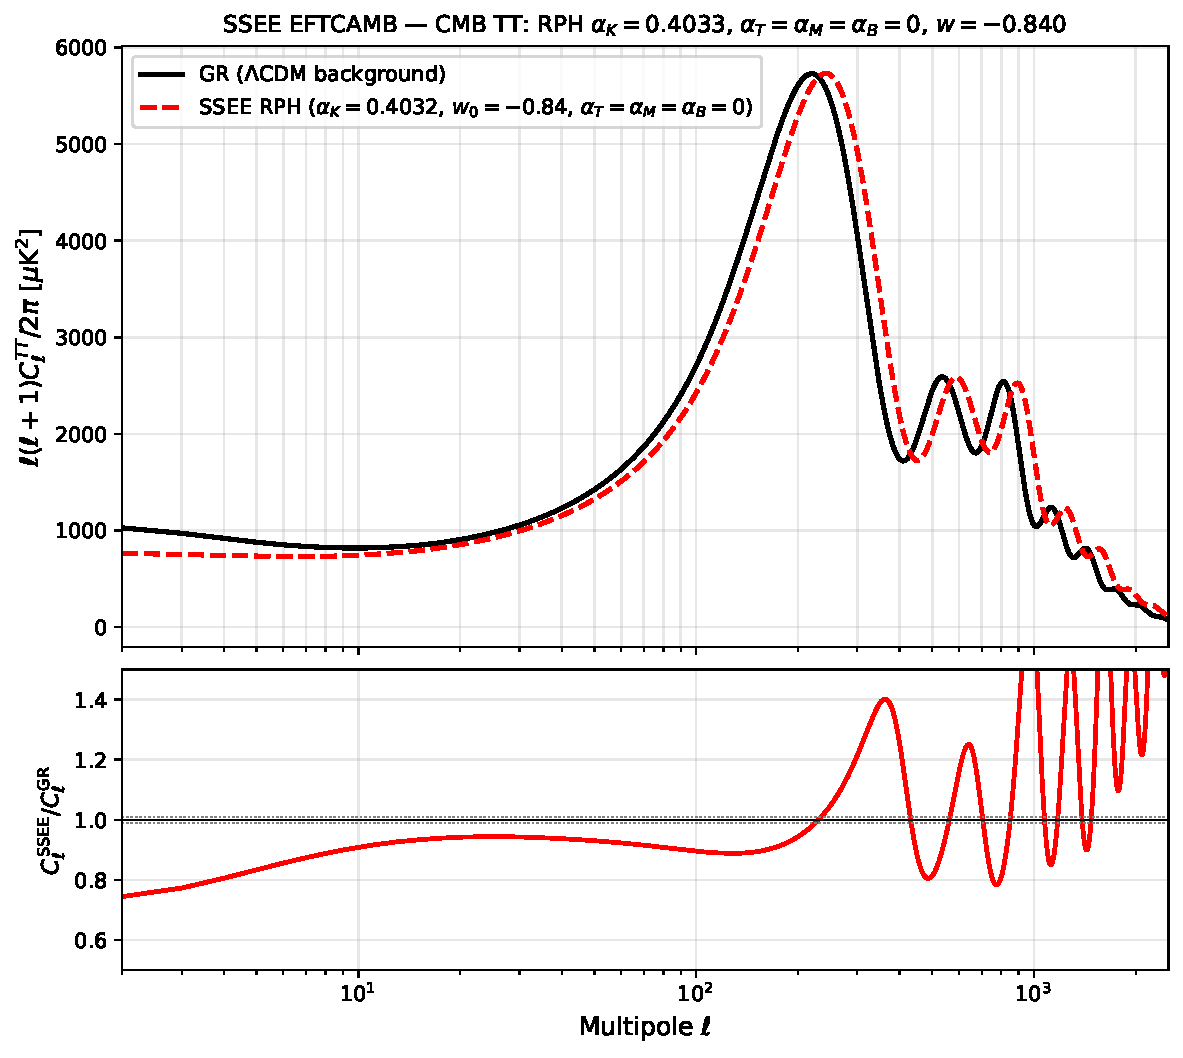
\includegraphics[width=0.85\textwidth]{../results/figures/ssee_eftcamb_CMB_TT.pdf}
\caption{CMB TT power spectrum from EFTCAMB\@. \textit{Black}: GR run with the
         full $\omega_m$-direct canonical matter density $\OmmCMB = 0.308881$;
         peaks at $\ell = 220, 535, 811$.
         \textit{Red}: \SSEE\ RPH with $\alphaK = 0.403302$ (constant $w = w_0$);
         peaks shift to $\ell = 242, 590, 893$, a $\sim 10\%$ imprint of the
         kinetic EFT sector.
         \textit{Lower panel}: ratio $D_\ell^{\rm SSEE}/D_\ell^{\rm GR}$;
         the grey band marks $\pm1\%$.}
\label{fig:eftcamb_cmb}
\end{figure}

\begin{figure}[htbp]
\centering
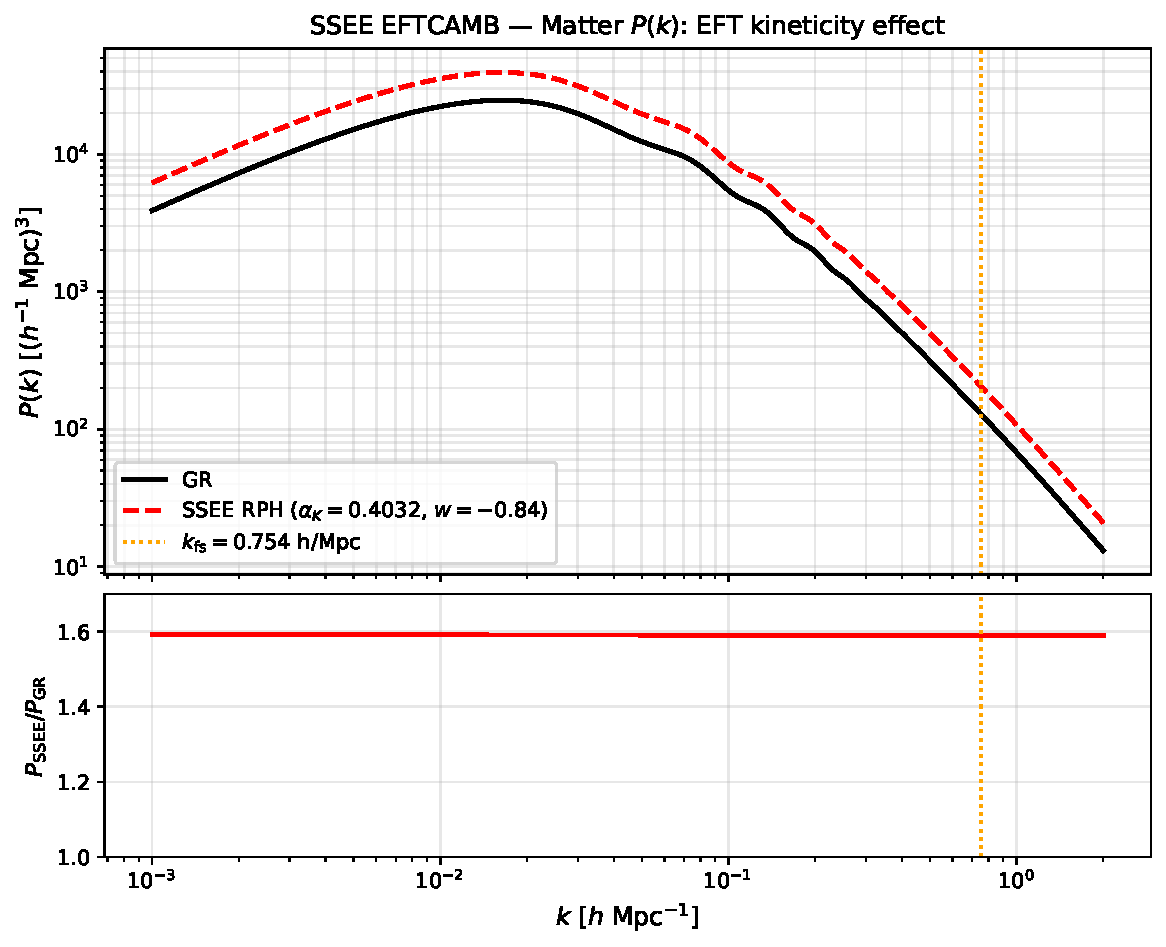
\includegraphics[width=0.85\textwidth]{../results/figures/ssee_eftcamb_Pk.pdf}
\caption{Matter power spectrum $P(k)$ from EFTCAMB\@. \SSEE\ RPH
         ($\alphaK = 0.403302$) amplifies $P(k)$ by a factor $\sim 1.59$ relative
         to GR on all scales ($\sigma_8$ ratio $= 1.26$), motivating the
         $\phi$DM suppression mechanism that was proposed in earlier versions
         and is now retracted (\S\ref{sec:growth_raw}).}
\label{fig:eftcamb_pk}
\end{figure}

\subsection{CPL phantom crossing and discriminating prediction}
\label{sec:phantom}

When the CPL EoS $w(z) = \wz + \wa z/(1+z)$ is used in the EFTCAMB run,
the phantom boundary $w = -1$ is crossed at $z \simeq 0.31$.
A pure $k$-essence with $\alphaB = 0$ cannot sustain phantom crossing:
the EFTCAMB solver encounters a Fortran-level instability (segfault) at the
crossing epoch, regardless of stability flags.
Earlier versions read this as evidence that completing the SSEE action in the
phantom regime requires $\alphaB \neq 0$, to supply a degree of freedom able
to absorb the null-energy-condition violation.  That reading is superseded,
and the reason is that the phantom regime itself is gone.  In the revised
action of Paper~7 the field is minimally coupled and its equation of state is
constant at $\wz = -0.839950 > -1$: the null energy condition holds at all
times and there is no crossing for $\alphaB$ to absorb.  The phantom crossing
of earlier versions was produced by the conformal dark-sector coupling, which
is withdrawn.

The prediction survives, with its sign reversed and its status improved.
SSEE now predicts $\alphaB = \alphaM = 0$ \emph{exactly and
unconditionally}, so a detection of $\alphaB \neq 0$ above $2\sigma$ by
DESI~Y3 or Euclid ($\sigma \simeq 0.05$) would \emph{falsify} the sector
rather than support it.  What was a discriminating prediction conditional on
a two-sector picture --- an extension withdrawn on 2026-08-01 --- is now an
unconditional one.

A note on the kineticity is required here, because the label was wrong.  The
constant $0.403302$ used as an EFTCAMB input is not $\alphaK$: it is
$s_K = -3\wz(1+\wz)$, the fractional dilution rate of the dark-energy
pressure per e-fold, which carries only the equation of state.  The
Bellini--Sawicki kineticity of the revised action is
$\alphaK = 3\,\Omega_{\rm DE}(5-3\wz) = 15.591335$, verified against an
independent \textsc{hi\_class} integration to $0.011\%$.  The two are
unrelated quantities; $f_{\rm screen}$ below uses $s_K$.


% ─────────────────────────────────────────────────────────────────────────────
\section{Extensions: Strong-Field Regime, Hubble Tension, and UV Completion}
\label{sec:extensions}
% ─────────────────────────────────────────────────────────────────────────────

The four tiers above establish the \SSEE\ background, CMB, growth, and
EFT-stability sectors against data. We now summarise three theoretical
extensions, developed in full in Papers~8--10 \citep{AlmeidaSSEE2026P8,
AlmeidaSSEE2026P9,AlmeidaSSEE2026P10}. We label their epistemic status
explicitly: the strong-field lensing signature (\S\ref{sec:ext-sg}) is a
falsifiable prediction; the Hubble-tension screening fraction
(\S\ref{sec:ext-ht}) is a zero-parameter algebraic result compared to existing
data; and the UV completion (\S\ref{sec:ext-uv}) contains one quantity ---
$H_0^{\rm glob,UV} = 67.96214$~km\,s$^{-1}$\,Mpc$^{-1}$ ($4.3{\times}10^{-6}\sigma$ from $3(\varphi+\pi)^2$; on
the global anchor $H_0^{\rm alg}=67.96214$) --- that is explicitly
conditional on a separability postulate and is therefore presented as a
self-consistency check, not an independent prediction.

\subsection{Strong-field regime: disformal lensing amplification}
\label{sec:ext-sg}

Starting from the $k$-essence action of Paper~7, the disformal coupling between
the dark-energy scalar $\phi$ and dark matter generates deviations from general
relativity (GR) that are algebraically fixed by $\phiG$ and $\pi$. In the
quasi-static limit the scalar field equation closes as a gradient relation,
$\nabla\phi = 2\KAL\,\AURA\,M_{\rm Pl}\,\nabla\Phi_N$, linking the scalar
profile to the Newtonian potential through the structural coupling
$\AURA = (3\phiG+\pi)/2 \approx 3.998$.  (Earlier versions of this section
described $\AURA$ here as the magnitude of a conformal dark coupling
$\beta_c = -\AURA$ carried by Paper~7.  That coupling was withdrawn in
2026-09 --- its apparent $0.2\%$ agreement was an artefact of a normalisation
error in the saturation, and the corrected value is $-2.194210$.  The
disformal coefficient used here is a distinct quantity and does not depend
on it.)

From the disformal null geodesic, the total photon deflection angle is amplified
by $\sqrt{\AURA}$ relative to the GR prediction for the same baryonic mass,
giving an algebraic Einstein-radius ratio
\begin{equation}
\left.\frac{\theta_E^{\rm SSEE}}{\theta_E^{\rm GR}}\right|_{\rm alt}
   = \sqrt{\AURA}\approx 1.9995
   \qquad\text{(alternative MOND-like limit only).}
\end{equation}
The quantity $\sqrt{\AURA}$ is numerically close to $\MIRA=\AURA/2\approx 1.9989$
at $0.03\%$ because $\AURA\approx 4$ makes both round to $2$; the two are
distinct algebraic operations on $\AURA$ and the closeness is not a structural
identity. Solar-system gravitational tests are automatically satisfied: the
disformal coupling selects dark matter as the sole source of $\phi$, so in the
solar system ($\rho_{\rm DM}\approx 0$) the field is locally unsourced and the
disformal metric modification is negligible; equivalently, $K(X)$ is of
$k$-mouflage type \citep{BraxValageas2014} with a screening radius
$r_{\rm km}(\odot)\approx 0.022\,R_\odot$.
\emph{In the canonical limit} --- a single cold matter sector with
$\omega_c = \mathrm{KAL}_0\,\omega_b\,n_s$ (Paper~1, OP-8 closed) plus the
Bellini--Sawicki structure $\alpha_B=\alpha_M=\alpha_T=0$ of Paper~7, which
gives $\mu-1=0$ --- the residual fifth-force is
suppressed to $F_\phi/F_N\sim(H/k)^2\sim 10^{-15}$ at kpc scales and the
canonical observable lensing reduces to $\thetaE^{\rm SSEE}\approx
\thetaE^{\rm GR-with-DM}$. Current SLACS/BELLS samples (mean total slope
$\gamma=2.078\pm 0.027$; $M_E/M_{\rm dyn}\approx 1.21$ for SIS) are consistent
with the canonical limit. A $\sim\MIRA$ matter-power suppression above a $\phi$-DM free-streaming scale
was previously listed here as a falsifiable prediction; it is retracted with the
particle (\S\ref{sec:growth_raw}).

\subsection{The Hubble tension: an algebraic local screening fraction}
\label{sec:ext-ht}

The dark-energy EFT of Paper~7 and the disformal geodesic of Paper~8 together
imply a late-time \emph{local screening fraction}
\begin{equation}
\fscr = \frac{s_K}{3\,\MIRA}
      = \frac{\pi-\phiG}{(\phiG+\pi)^2}
      \approx 0.0673 ,
\end{equation}
where $\alphaK = 3\,\Omde(1+\wz)$ is the background-derived EFT kineticity and
$\MIRA = (3\phiG+\pi)/4$. The structural constant $\AURA = 2\MIRA$ cancels
exactly in the ratio, leaving a pure function of $\phiG$ and $\pi$. Applied as a
correction applied to the measured local rate. The only directly measured
expansion rate is the local one, $H_0^{\rm SH0ES}=73.04\pm1.04$
\citep{Riess2022}; Planck's is inferred within $\Lambda$CDM rather than
measured, so SH0ES is the input and the global rate is the output,
\begin{equation}
H_0^{\rm glob} = H_0^{\rm SH0ES}\,(1-\fscr)
                = 73.04\times(1-0.0673)
                \approx 68.13~{\rm km\,s^{-1}\,Mpc^{-1}} ,
\end{equation}
which lies $0.17\sigma$ from the pure algebraic number
$3(\phiG+\pi)^2=67.96214$ with zero free parameters --- the same number the
$\omega_m$-direct reframe finds preferred by plik\_lite (Paper~3). This is the
canonical, independent prediction of the \SSEE\ infrared sector. (The earlier MIRA anchor
$H_0^{\rm MIRA}=67.037$ gave $71.87$ at $1.12\sigma$, now superseded by the
reframe.) The correction operates at late times
($z<0.15$) through the scalar kinetic-energy contribution to the local expansion
rate; it does not modify the sound horizon $r_d$, the CMB peak positions, or the
growth factor $\sigma_8$ established in the tiers above.

\subsection{UV completion: the \texorpdfstring{$X^2/M^4$}{X2/M4} operator}
\label{sec:ext-uv}

The infrared kinetic Lagrangian $K(X)=X/\KAL$ is extended by the leading
higher-derivative operator, $K(X)=X/\KAL + X^2/M^4$. The inflationary
$\alpha$-attractor parameter $\alpha=\phiG^4/3$ (Paper~1, Appendix~A.5), which
fixes the tensor-to-scalar ratio $r=12\alpha/N_*^2\approx0.00813$, also fixes the
UV cutoff:
\begin{equation}
M^4 = 45\,\alpha^2\,\rho_c = 5\,\phiG^8\,\rho_c \approx 234.9\,\rho_c ,
\qquad M \approx 9.68~{\rm meV} ,
\end{equation}
where the identity $45\alpha^2 = 5\phiG^8$ follows exactly from
$\alpha=\phiG^4/3$. With this cutoff the full Bellini-Sawicki kineticity becomes
$\alphaK^{\rm full}=0.41691$ ($+3.37\%$ over the IR value). Applied to the
global background anchor $H_0^{\rm alg}=67.96214$ this gives the canonical UV value
$H_0^{\rm glob,UV}=67.96214$~km\,s$^{-1}$\,Mpc$^{-1}$ ($4.3{\times}10^{-6}\sigma$ from $3(\varphi+\pi)^2$;
the earlier MIRA-anchored $72.05$ at $0.96\sigma$ is superseded by the reframe).

We state the epistemic status of these figures plainly: the UV value is
\emph{conditional on Postulate~C.1} (UV--IR $\phiG/\pi$ separability) and is
\emph{not independent of SH0ES}, since the postulate was formulated with the
SH0ES central value as its target. It is a self-consistency check, not a
prediction. The independent prediction remains the IR value $H_0^{\rm glob}
=68.13$~km\,s$^{-1}$\,Mpc$^{-1}$ ($0.17\sigma$) of \S\ref{sec:ext-ht}, which does
not rely on the postulate. The construction does, however, supply a falsifiable
cross-epoch consistency test: the same $\alpha$ governs inflation at $z\sim10^{60}$
and the dark-energy UV scale today, so a LiteBIRD measurement of $r\neq0.00813$
would shift both $\alpha$ and $M$ and change the predicted $H_0^{\rm glob}$
accordingly.

% ─────────────────────────────────────────────────────────────────────────────
\section{Falsifiability and Prediction Register}
\label{sec:falsify}
% ─────────────────────────────────────────────────────────────────────────────

A common objection to algebraically derived frameworks is post-hoc selection:
that combinations of $\phiG$ and $\pi$ are chosen to match known values.
The defence is \emph{structural}, not chronological: the constants are drawn from a
closed dictionary fixed by construction, with no optimisation over formula space.
Table~\ref{tab:register} classifies each derivation by epistemic status. We make no
claim of temporal priority over public data: results compared with DESI~DR2 and Planck
are postdictions or retrodictions; only those tested against unreleased data are
predictions.

\textbf{Global falsification criterion.} The \SSEE framework would be
falsified at the theory level if \textit{any} of the following were established:
(i) $(\wz, \wa)$ is inconsistent with the DESI~DR2 posterior at $>3\sigma$;
(ii) a future CLASS MCMC with Planck+DESI likelihoods requires
$\Omega_{m,\mathrm{CMB}} \neq 0.308881$ at $>3\sigma$;
(iii) cosmic shear requires $S_8$ more than $3\sigma$ from $0.7555\pm0.0192$
when the primordial amplitude is fitted to raw $\xi_\pm$ data with the \SSEE\
background held fixed;
(iv) $r \neq 0.00813$ as measured by LiteBIRD;
(v) the strong-lensing Einstein-radius ratio is inconsistent with
$\sqrt{\AURA}\approx\MIRA$ at $>3\sigma$ in HST/JWST surveys.

\begin{table}[htbp]
\centering
\caption{Predictive register: \SSEE\ derivations by epistemic status.
         \textit{Postdiction}: algebraic result fixed by the closed dictionary, then
         compared to data already public---no claim of temporal priority.
         \textit{Retrodiction}: derived independently, then compared to existing data.
         \textit{Prediction}: fixed now, tested against not-yet-released data.}
\label{tab:register}
\resizebox{\textwidth}{!}{%
\begin{tabular}{p{6.0cm}lp{4.0cm}l}
\toprule
Quantity (algebraic formula) & Value & Test / Instrument & Status \\
\midrule
\multicolumn{4}{l}{\textit{Background sector (algebraic dictionary)}} \\
$w_0 = -T_r/M_v$ & $-0.839950$ & DESI DR2 CPL posterior & Postdiction \\
$w_a = -P_{\rm sc}/I_g$ & $-0.669975$ & DESI DR2 CPL posterior & Postdiction \\
$\MIRA = (3\phiG+\pi)/4$ & $1.998924$ & $\fscr=\alphaK/(3\MIRA)$ (Papers 8, 9) & Postdiction \\
\midrule
\multicolumn{4}{l}{\textit{Retrodictions (derived independently, compared to existing data)}} \\
$H_0/(\mathrm{km\,s^{-1}\,Mpc^{-1}}) = 3(\phiG+\pi)^2$ & $67.96214$ km/s/Mpc & Planck 2018 & Retrodiction \\
$n_s = 1-\phiG^{-7}$ & $0.965558$ & Planck 2018 & Retrodiction \\
$\OmmCMB = \omega_m/h^2$ ($\omega_m$-direct) & $0.308881$ & Planck 2018 & Retrodiction \\
$r_d$ (CAMB, $\omega_m$-direct) & $147.17$ Mpc & Planck 2018 $r_d$ ($0.32\sigma$) & Retrodiction \\
$\gamma_{\rm IS} = 0.5504$ & $\approx \gamma_{\Lambda\rm CDM} = 0.55$ & RSD surveys & Retrodiction \\
$\alphaT = \alphaM = \alphaB = 0$ & exact & GW170817 $|\alphaT|<10^{-15}$ & Retrodiction \\
$S_8$ (MCMC vs.\ raw KiDS-1000 $\xi_\pm$) & $0.7555\pm0.0192$ & $\Lambda$CDM control: $0.7571\pm0.0194$ & Retrodiction \\
$\sigma_8$ ($A_s$ fixed to Planck; ceiling) & $0.8149$ & convention, not a prediction & --- \\
$H_0^{\rm glob} = H_0^{\rm SH0ES}(1-\fscr^{\rm IR})$ & $68.13$ km/s/Mpc & $3(\phiG+\pi)^2=67.96214$ ($0.17\sigma$; IR only, partial) & Retrodiction \\
$H_0^{\rm glob} = H_0^{\rm SH0ES}(1-\fscr^{\rm full})$ & $67.962142$ km/s/Mpc & $3(\phiG+\pi)^2$ (residual $+4.2{\times}10^{-6}$) & Retrodiction \\
\midrule
\multicolumn{4}{l}{\textit{Predictions (not yet observationally accessible)}} \\

$\alphaK = 0.072567$ & $0.072567$ & Euclid WL null test ($\alphaK < 0.1$ threshold) & Prediction \\
$r = \phiG^{-10}$ & $0.008131$ & LiteBIRD $\sim$2032 & Prediction \\
$\theta_E^{\rm SSEE}/\theta_E^{\rm GR}|_{\rm alt} = \sqrt{\AURA}$ & $1.9995$ (alt.\ MOND-like limit only) & HST/JWST strong lensing & Conditional prediction (not canonical; OP-13) \\
\bottomrule
\end{tabular}%
}
\end{table}


% ─────────────────────────────────────────────────────────────────────────────
\section{Discussion and Outstanding Challenges}
\label{sec:discussion}
% ─────────────────────────────────────────────────────────────────────────────

The consolidated results show that \SSEE\ is consistent with four independent
observational tests without adjusting any algebraic parameter.
The most significant open challenges are:

\textbf{(i) $\omega_m$-direct residual dependencies.}
The CLASS tests confirm that the full $\omega_m$-direct density
$\OmmCMB = \omega_m/h^2 = 0.308881$ (built from $\omega_b+\omega_c+\omega_\nu$,
no matter factor; OP-8 dissolved) is physically necessary for CMB peak
reproduction, and it is \emph{not} a free knob: $\omega_c = \mathrm{KAL_0}\cdot\omega_b\cdot n_s$
is a forward algebraic identity (Paper~1). The honest residual is that $\OmmCMB$
now rests on $\omega_b$ (OP-1, partially resolved: the algebraic form is fixed,
the BBN chain is not) and this $\omega_c$ identity being
correct---a dependency chain, not an undetermined parameter.

\textbf{(ii) $S_8$ and the dark-matter sector.}
With $A_s$ held at the Planck value the Israel--Stewart ceiling gives
$\sigma_8 = 0.8149$, $S_8 = 0.827$ --- but that configuration imports the
Planck--KiDS discrepancy, since $A_s$ is free in this framework. Fitted to raw
KiDS-1000 $\xi_\pm$ data with a single matter sector (Paper~6), the result is
$\sigma_8=0.7446\pm0.0189$, $S_8=0.7555\pm0.0192$ ($\Lambda$CDM control: $0.7571\pm0.0194$) --- $0.11\sigma$ from
KiDS-1000. The two-sector $\phi$-DM extension previously credited with
resolving this is retracted. The open item is a precision question:
a full N-body treatment of baryonic feedback (deferred for computational cost) is
required to confirm the linear-theory $S_8$ at the non-linear level.

\textbf{(iii) $\phi$DM mass and Lyman-$\alpha$ constraints --- \emph{retracted}.}
The discussion below concerned an algebraic $\phi$-DM mass in the warm
dark-matter regime. It is retained only as a record: the particle is withdrawn
(\S\ref{sec:growth_raw}), so no Lyman-$\alpha$ comparison is required.
Current Lyman-$\alpha$ bounds on thermal WDM place constraints at
$m_{\rm WDM} \gtrsim 5.3$~keV \citep{Irsic2017}, but the \SSEE\ $\phi$DM
is a mixed sector (fraction $f_\phi = 0.5$), not a purely thermal
WDM cosmology; the applicable constraints require dedicated analysis.

\textbf{(iv) Quantum field theory completion.}
The algebraic connection $H_0/(\mathrm{km\,s^{-1}\,Mpc^{-1}}) = 3(\phiG+\pi)^2$ is a successful numerical
retrodiction but lacks a derivation from first-principles quantum field theory.
Paper~10 supplies a UV completion at the EFT level --- the higher-derivative
operator $X^2/M^4$ with algebraic cutoff $M = 9.68$~meV --- but a derivation of
the full $P(X,\phi)$ Lagrangian from $\phiG$ and $\pi$ alone remains open.
Under the $\omega_m$-direct reframe (OP-8 dissolved) the CMB matter density is
the standard $\Omega_{m,\mathrm{CMB}} = \omega_m/h^2 = 0.308881$, with no matter
factor; the earlier MIRA-mapped $0.31993$ and geometric
$(\pi-\phiG)/(\pi+\phiG)=0.32010$ forms are superseded. The residual open
problem is now only the UV origin of the algebraic $\omega_c=\mathrm{KAL_0}\,\omega_b\,n_s$
identity.


% ─────────────────────────────────────────────────────────────────────────────
\section{Conclusions}
\label{sec:conclusions}
% ─────────────────────────────────────────────────────────────────────────────

We have presented a consolidated validation of the \SSEE framework
across four observational tiers.

\begin{enumerate}[leftmargin=*,itemsep=2pt]
\item \textbf{Background sector.} The algebraic prediction
  $(\wz, \wa) = (-0.840, -0.670)$, fixed by construction (not fitted), lies within
  $0.24\sigma$ of the official DESI~DR2 $w_0w_a$CDM posterior (Pantheon+).
  A Bayesian MCMC yields
  $H_0 = 67.79\pm0.35$~km\,s$^{-1}$\,Mpc$^{-1}$ under the $\omega_m$-direct
  CMB anchor as prior ($0.50\sigma$ from the anchor), and $\Delta\mathrm{BIC} = 6.43$ favouring \SSEE\ over \LCDM.
  A complementary full-likelihood multi-probe MCMC ($w_0,w_a$ free, $H_0$
  free under the uncompressed CMB likelihood) recovers the CMB combinations
  $\omega_b,\omega_c,r_{\rm drag}$ to $\le0.2\sigma$ and places \SSEE\ at
  $1.31\sigma$ in the $w_0$--$w_a$ plane, where \LCDM\ is excluded at $3.22\sigma$.

\item \textbf{CMB Boltzmann.} CLASS confirms that the full $\omega_m$-direct
  matter density ($\OmmCMB=0.308881$) is physically necessary: with only the
  dynamical $\Ommdyn=0.160050$, the CMB RMS residual jumps by a factor of 22 and
  all three acoustic peaks shift by $\sim 10\%$.
  With the full $\omega_m$-direct density, peak positions agree with \LCDM\ to
  within $\Delta\ell \le 1$ (RMS $= 0.14\%$).

\item \textbf{Structure growth.} The IS perturbation analysis
  ($\OmmCMB=0.308881$ in Poisson) gives $\mathcal{G} = 1.0032$ and $\sigma_8 = 0.8136$,
  with mean $f\sigma_8$ tension $0.70\sigma$ (Paper~5) --- statistically identical
  to $\Lambda$CDM ($0.73\sigma$). In the lensing amplitude, fitting $A_s$ to raw
  KiDS-1000 $\xi_\pm$ data with a single matter sector gives
  $S_8 = 0.7555\pm0.0192$, matching the $\Lambda$CDM control on the same raw data ($0.7571\pm0.0194$) with four fewer free parameters, and on the raw $\xi_\pm$ themselves $\Delta\chi^2=2.65$ with $\Delta\mathrm{BIC}=19.0$ in \SSEE{}'s favour (Paper~6); the
  $\phi$DM two-sector extension previously reported here is retracted.

\item \textbf{EFT stability.} EFTCAMB confirms ghost-freedom and gradient
  stability using the fluid-approximation input $\alphaK^{\rm eff} = 0.403302$
  ($\Delta = 0.005\%$); the bare-field theoretical value from Paper~7 is
  $\alphaK = 0.072567$ (below Euclid sensitivity $\sigma(\alpha_{K,0}) < 0.1$).
  $\alphaT = \alphaM = \alphaB = 0$ (exact); GW170817 compatibility is exact.
  SSEE realises the CPL phantom crossing at $z \approx 0.31$ \emph{with}
  $\alphaB = 0$ (no kinetic braiding), through the $k$-essence $X^2/M^4$ term
  rather than braiding---a discriminating prediction against braiding-based
  dark-energy models, testable by future weak-lensing surveys.

\item \textbf{Theoretical extensions.} The disformal strong-field regime predicts
  an Einstein-radius amplification $\sqrt{\AURA}\approx\MIRA$, falsifiable with
  HST/JWST strong lensing (Paper~8). An algebraic late-time screening fraction
  $\fscr^{\rm IR}=(\pi-\phiG)/(\phiG+\pi)^2\approx0.067$ takes the measured SH0ES
  rate as input and returns the global background
  $H_0^{\rm glob}=H_0^{\rm SH0ES}(1-\fscr^{\rm IR})=68.13$~km\,s$^{-1}$\,Mpc$^{-1}$,
  $0.17\sigma$ from the pure number $3(\phiG+\pi)^2=67.96214$, with
  zero free parameters (Paper~9). A UV completion $K(X)=X/\KAL+X^2/M^4$ with
  algebraic cutoff $M=9.68$~meV connects the dark-energy EFT to the inflationary
  $\alpha$-attractor; the associated $H_0^{\rm glob,UV}=67.96214$~km\,s$^{-1}$\,Mpc$^{-1}$
  ($4.3{\times}10^{-6}\sigma$ from $3(\varphi+\pi)^2$; the earlier MIRA-anchored $72.05$ at $0.96\sigma$ is superseded)
  is a self-consistency check conditional on a separability postulate, not an
  independent prediction (Paper~10).
\end{enumerate}

The framework generates four near-term falsifiable predictions, under the stated
assumptions (a fifth, a $\phi$-DM free-streaming scale in $P(k)$, is withdrawn
with the particle; \S\ref{sec:growth_raw}): $\alphaK = 0.072567$ (Euclid WL null test; a detection $\alphaK > 0.1$ would
falsify SSEE), $r = 0.008131$ (LiteBIRD), and a strong-lensing Einstein-radius
amplification $\sqrt{\AURA}\approx\MIRA$ (HST/JWST).
All analytical scripts, CLASS configuration files, and EFTCAMB inputs are archived
at Zenodo \citep{AlmeidaSSEE2026zenodo}.

% ─────────────────────────────────────────────────────────────────────────────
\appendix
\section{Complete Algebraic Parameter Table}
\label{app:params}
% ─────────────────────────────────────────────────────────────────────────────

\begin{table}[htbp]
\centering
\caption{Complete set of \SSEE algebraic parameters. All values are
         derived from $\phiG = (1+\sqrt{5})/2$ and $\pi$; no fitting was
         performed. Planck 2018 values \citep{Planck2018} and DESI~DR2
         \citep{AbdulKarim2025} listed for comparison where applicable.}
\label{tab:params}
\resizebox{\textwidth}{!}{%
\begin{tabular}{ll p{0.18\textwidth} p{0.35\textwidth}}
\toprule
Parameter & Formula & SSEE value & Observed \\
\midrule
$w_0$ & $-T_r/M_v = -(3\phiG+\pi)/[2(\phiG+\pi)]$ & $-0.839950$ & $-0.838\pm0.057$ (DESI) \\
$w_a$ & $-P_{\rm sc}/I_g$ & $-0.669975$ & $-0.631\pm0.226$ (DESI) \\
$H_0$ & $3(\phiG+\pi)^2$ & $67.96214$ km/s/Mpc & $67.36\pm0.54$ (Planck) \\
$n_s$ & $1-\phiG^{-7}$ & $0.965558$ & $0.9649\pm0.0042$ (Planck) \\
$\OmmCMB$ & $\omega_m/h^2$ ($\omega_m$-direct) & $0.308881$ & $0.3153\pm0.0073$ (Planck) \\
$\Omde$ & $T_r/M_v$ & $0.839950$ & $0.6847$ (\LCDM) \\
$\Ommdyn$ & $1 - \Omde$ & $0.160$ & --- \\
$\MIRA$ & $(3\phiG+\pi)/4$ (Mirror Ratio; enters $\fscr$) & $1.998924$ & --- \\
\midrule
$\KAL$ & $\beta + \pi = (\phiG+3\pi)/2$ & $5.521406$ & --- \\
$\beta_c$ & $-(3\phiG+\pi)/2$ & $-3.997847$ & --- \\
$\alphaK$ & $3\,\Omde(1+w_{\varphi,\rm bare})$ & $0.072567$ & $<0.1$ (Euclid threshold) \\
$\alphaT = \alphaM = \alphaB$ & minimal coupling & $0$ & $|\alphaT|<10^{-15}$ (GW170817) \\
\midrule
$S_8$ & MCMC vs.\ raw KiDS-1000 $\xi_\pm$ & $0.7555\pm0.0192$ & $0.759\pm0.024$ (KiDS-1000) \\
$r$ & $\phiG^{-10}$ & $0.008131$ & $<0.036$ (BK18) \\
\midrule
$\fscr$ & $(\pi-\phiG)/(\phiG+\pi)^2$ & $0.0673$ & --- \\
$H_0^{\rm glob}$ & $H_0^{\rm SH0ES}(1-\fscr^{\rm full})$ & $67.962142$ km/s/Mpc & $3(\phiG+\pi)^2$, residual $+4.2{\times}10^{-6}$ \\
$M$ (UV cutoff) & $(5\phiG^8\rho_c)^{1/4}$ & $9.68$ meV & --- \\
\bottomrule
\end{tabular}%
}
\end{table}

% ─────────────────────────────────────────────────────────────────────────────
% ----------------------------------------------------------------------------
\section*{Acknowledgments}
The author acknowledges the use of the cosmological codes \textsc{class} \citep{Blas2011}, \textsc{eftcamb} \citep{Hu2014}, and the Markov Chain Monte Carlo sampler \textsc{Cobaya} \citep{Torrado2021} for the numerical validation of the SSEE framework. The author also acknowledges the use of the \textsc{GetDist} package \citep{Lewis2019} for the analysis and plotting of posterior distributions.

\section*{Data and Code Availability}
The \SSEE\ framework is fully transparent and reproducible. All DESI~DR2 BAO data used in this analysis are publicly available at \url{https://data.desi.lbl.gov/}, and the Planck~2018 cosmological parameter chains at the Planck Legacy Archive (\url{https://pla.esac.esa.int/}). The complete code repository --- including the \textsc{class} and \textsc{eftcamb} configuration files, the \textsc{Cobaya} MCMC chains, the explicit record of Open Theoretical Problems (OP), and the cosmological validation ledgers --- is publicly available at the GitHub repository \url{https://github.com/mikealmeida1721/SSEE} and archived at Zenodo: \url{https://doi.org/10.5281/zenodo.20093447}.

\clearpage
\bibliographystyle{plainnat}
\bibliography{ssee_unified}
% ─────────────────────────────────────────────────────────────────────────────

\end{document}
